\documentclass[12pt, a4paper, oneside]{ctexart}
\usepackage{amsmath, amsthm, amssymb, graphicx}
\usepackage[bookmarks=true, colorlinks, citecolor=blue, linkcolor=black]{hyperref}
\usepackage[margin = 25mm]{geometry}
\usepackage{setspace}
\usepackage{listings}
\usepackage{ctex}
\usepackage{cite}
\usepackage{float}
\usepackage{xcolor}
\usepackage{amsmath}
\definecolor{codegreen}{rgb}{0,0.6,0}
\definecolor{codegray}{rgb}{0.5,0.5,0.5}
\definecolor{codepurple}{rgb}{0.58,0,0.82}
\definecolor{backcolour}{rgb}{0.95,0.95,0.92}

\lstdefinestyle{mystyle}{
    backgroundcolor=\color{backcolour},   
    commentstyle=\color{codegreen},
    keywordstyle=\color{magenta},
    numberstyle=\tiny\color{codegray},
    stringstyle=\color{codepurple},
    basicstyle=\ttfamily\footnotesize,
    breakatwhitespace=false,         
    breaklines=true,                 
    captionpos=b,                    
    keepspaces=true,                 
    numbers=left,                    
    numbersep=5pt,                  
    showspaces=false,                
    showstringspaces=false,
    showtabs=false,                  
    tabsize=2
}

\lstset{style=mystyle}


\title{Lennard-Jones势能下的液氩模拟暨GROMACS软件学习报告}
\date{\today}
\author{202011010101物理2001孙陶庵}
\begin{document}
\begin{spacing}{2.0}
\tableofcontents
\maketitle
\section{事前声明}
GROMACS是之前完全没有接触过的东西,连安装都不是执行档(exe),遇到了非常多的困难;我在网络上找到了马普所的Prof. Bert de Groot写得一篇文章\cite{NBS_2021},就是直接和这次大作业的主题对上的。
该文章的前半部分讲得是气体的拟合,后半部分讲得是液体部分的。因为网络上的教程太过于稀少(无论中英文),就算有,也是又臭又长的影片,根本无法在一周之内学习完然后完成报告,所以只能使用这位教授的源代码,只做学习之用绝无抄袭之意。
我以下这些东西基本都是使用这位教授的源代码,以作为学习之用,绝无抄袭之意图,但同时本文中讨论的部分以及分析结果的部分都是自己搜集资料查询并得出的结果。
使用软件:\\
1.GROMACS\\
2.Pymol\\
3.python
\section{Lennard-Jones势能模型}
$V(r)=4\epsilon\left[\left(\frac{\sigma}{r}\right)^{12}-\left(\frac{\sigma}{r}\right)^6\right]$
其中,$V(r) $表示两个粒子之间的势能,$\epsilon$表示势能的深度参数,$\sigma$表示粒子间的距离参数,r 表示两个粒子之间的距离。

模型的物理解释:
\\
1.斥力项:第一项$\left(\frac{\sigma}{r}\right)^{12}$表示斥力项,它随着粒子之间距离的减小而迅速增大。这一项源于泡利不相容原理,即两个粒子之间的电子云不能重叠。
当两个粒子靠得很近时,由于泡利不相容原理的限制,电子云之间的排斥力急剧增加,导致斥力项迅速增大,使得粒子之间发生排斥作用。
这一项的存在可以解释为什么物质的体积是有限的,因为当粒子之间的距离趋近于零时,斥力项趋近于正无穷大,使得粒子无法进一步靠近。\\
2.引力项:第二个项$\left(\frac{\sigma}{r}\right)^6$表示引力项,它随着粒子之间距离的减小而迅速减小。这一项源于分子之间的范德华力,即分子之间由于电荷分布产生的吸引力。
当两个粒子之间的距离较大时,引力项占主导地位,使得粒子之间发生吸引作用。然而,随着距离的减小,斥力项的贡献逐渐增大,抵消了引力项的作用,
导致势能逐渐减小。这一项的存在可以解释为什么物质在一定范围内具有吸引力,导致分子能够聚集成液体或固体的形态。

\section{问题}

使用gromacs在windows环境下进行液氩模拟实验\\
1.设定液氩系统的模拟参数。参数包括:氩原子数量,模拟箱的尺寸,温度,模拟总时间和步长等\\
2.使用Lennard-Jones势能描述氩原子的相互作用,进行液氩的分子动力学模拟\\
3.记录模拟过程中的数据,包括系统的能量温度压强等物理量的时间演化\\
4.分析结果,解释模拟结果的物理意义,并于理论预测结果相比较\\
\section{初始文件设置}
\subsection{设定拓扑文件(argon.top)}
\begin{lstlisting}[caption={argon.top}]
    [ defaults ]
; nbfunc        comb-rule       gen-pairs       fudgeLJ fudgeQQ
  1             1               no              1.0     1.0

[ atomtypes ]
AR  39.948    0.0   A     0.00622127     9.69576e-06

[ moleculetype ]
; molname       nrexcl
Ar              1

[ atoms ]
; id    at type res nr  residu name     at name  cg nr   charge
1       AR       1       Ar              Ar        1       0

[ system ]
; Name
Argon

[ molecules ]
; Compound        #mols
AR                216
\end{lstlisting}
其中[ atomtypes ]里面的A项(0.0后面0.00622127前面)即为Lennard-Jones势能在gromacs的代号
\subsection{设定结构文件(liquid.gro)}
总共219行的参数文件,参见附件
\subsection{设定分子动力学参数(94k.mdp)}
总共217行的参数文件,参见附件
包含初始条件及其它参数
\section{编译-结果-及分析}
分别输入以下命令:
\begin{lstlisting}
    gmx grompp -f 94k.mdp -c liquid.gro -p argon.top
    gmx mdrun -v -c liquid.pdb -nice 0
    gmx msd -s -o msd.xvg -f traj_comp.xtc -trestart 50 -b 100
\end{lstlisting}
并且设定完全后,会得到xvg档案,我们使用python分析画图
\begin{figure}[H]
    \begin{minipage}[t]{0.5\linewidth}
        \centering
        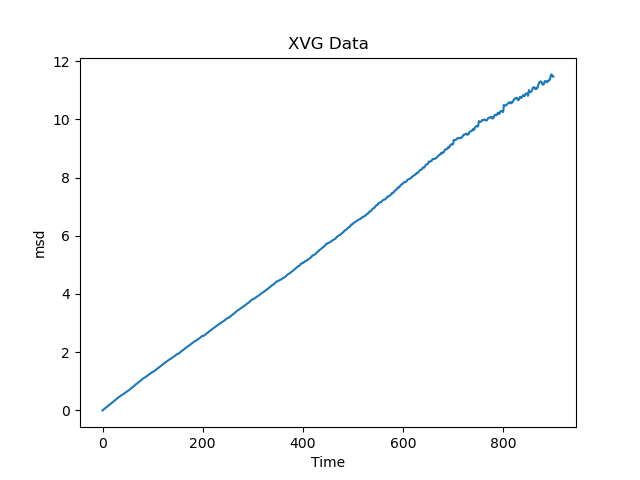
\includegraphics[scale=0.3]{msdxvg.png}
        \caption{结果}
        \label{fig:side:a}
      \end{minipage}%
      \begin{minipage}[t]{0.5\linewidth}
        \centering
        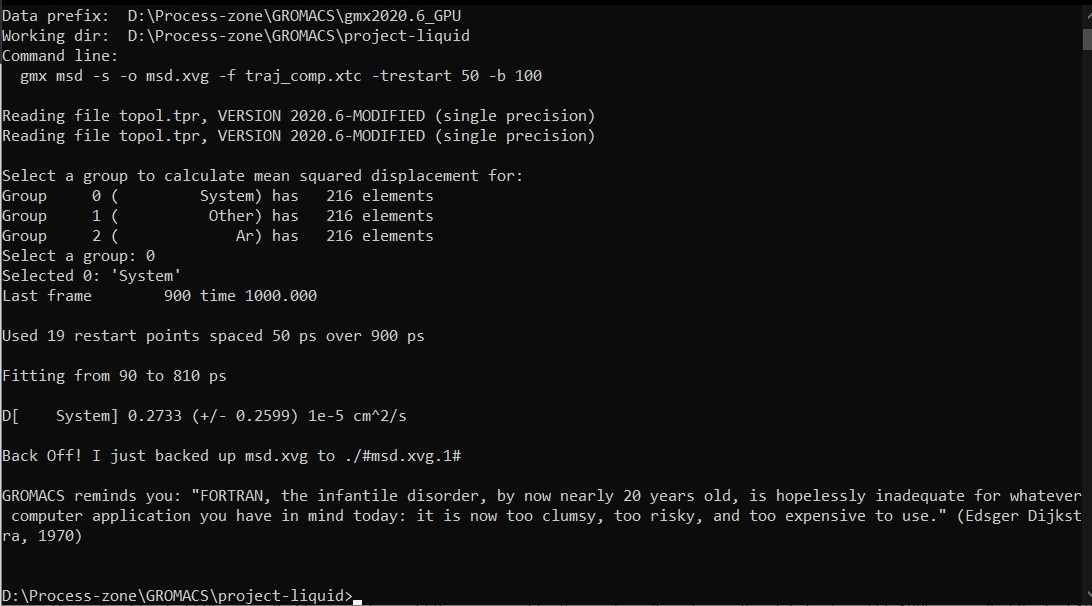
\includegraphics[scale=0.3]{msdxvgworking.jpg}
        \caption{得到扩散系数$2.1853\times 10^{-5}cm^2/s$}
        \label{fig:side:b}
      \end{minipage}
\end{figure}

\section{分子模拟}
\begin{lstlisting}
    wget http://www3.mpibpc.mpg.de/groups/de_groot/compbio1/p1/anneal2.mdp
    gmx grompp -f anneal2.mdp -c liquid.gro -p argon.top -maxwarn 1
    gmx mdrun -v -c anneal2.pdb -nice 0
\end{lstlisting}
以上指令用于跑(mdrun)出拟合档案liquid.gro(结构文件)及 traj\_comp.xtc(轨迹文件)
将以上这两个文件放在Pymol中打开后会得到一段分子振动的影片,并将其打印成GIF档(见附件)
\section{径向分布函数(RDF)分析}
RDF可以提供有关系统中粒子之间的距离分布信息。分析RDF可以确定粒子之间的最近邻距离、平均距离以及周期性结构(如晶体中的晶格常数)同时也可以研究相变过程。
相变通常涉及粒子的聚集或分散,以及结构的变化。通过监测RDF随温度、压力或其他条件的变化,可以探索相变过程中粒子的聚集行为。
接下来讨论如何使用rdf来分析:
\begin{figure}[H]
    \begin{minipage}[t]{0.5\linewidth}
        \centering
        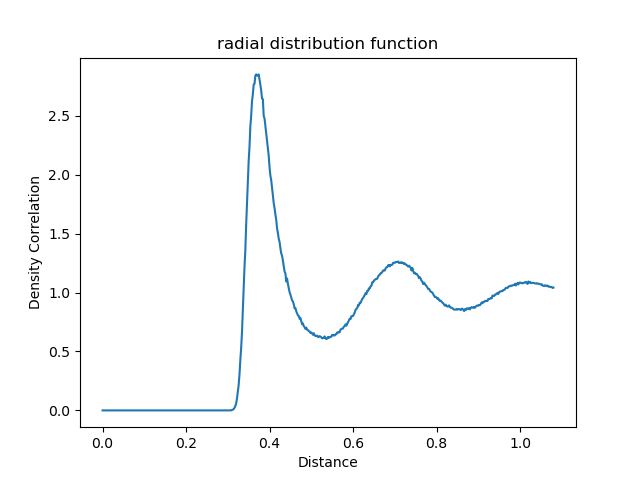
\includegraphics[scale=0.5]{radial distribution function.png}
        \caption{liquid}
        \label{fig:side:a}
      \end{minipage}%
      \begin{minipage}[t]{0.5\linewidth}
        \centering
        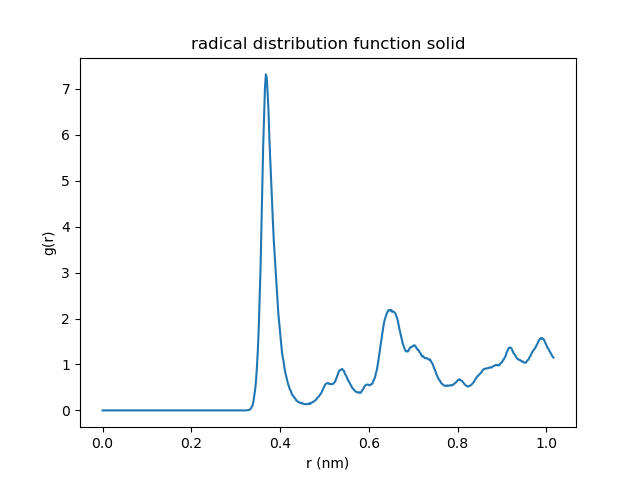
\includegraphics[scale=0.5]{radial distribution function solid.png}
        \caption{solid}
        \label{fig:side:b}
      \end{minipage}
\end{figure}


通过模拟液态氩和固态氩的系统,可以观察和比较两种相态的结构和性质。液态氩的原子会存在较大的自由度和较弱的相互作用,而固态氩的原子会排列成有序的晶格结构,并具有较强的相互作用。
固体部分在r=0.4 nm时达到了约7左右的极端值,而液体部分只有不到3。这说明在固体相中,在距离为0.4 nm的位置上,原子之间存在更强烈的相互作用或者更密集的排列。
这大概是因为固体和液体的结构差异。在固体中,原子通常排列成紧密的晶格结构,原子之间的相互作用力更强,因此在g(r)函数中会观察到较高的峰值。
而在液体中,原子之间的排列相对更为松散,相互作用力较弱,因此在g(r)函数中的峰值较低。
\begin{figure}[H]
	\centering
	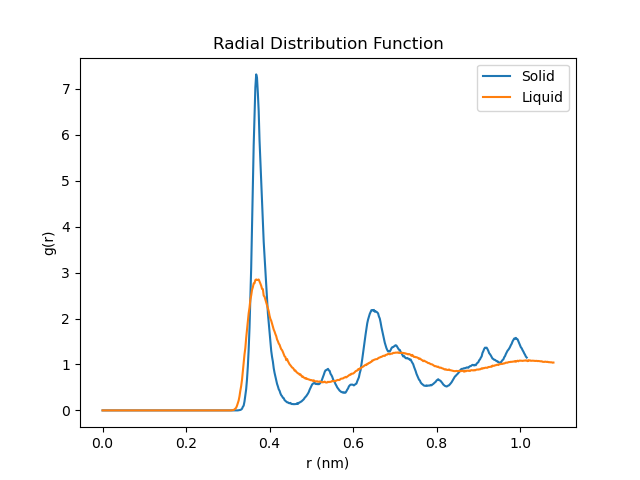
\includegraphics[width=8cm]{Radial Distribution Function2.png}
	\caption{all in one}
\end{figure}

\section{数据处理}
\subsection{表格数据分析}
我们从日志文件(md.log)中可以找到软件对数据的记录:
\begin{center}
  Energies (kJ/mol)
  \begin{table}[h]
    \centering
    \begin{tabular}{|c|c|c|c|c|}
    \hline
    LJ (SR) & Disper. corr. & Coulomb (SR) & Potential & Kinetic En. \\
    \hline
    $-1.06112 \times 10^{3}$ & $-1.86835 \times 10^{2}$ & $0.00000$ & $-1.24795 \times 10^{3}$ & $2.22800 \times 10^{2}$ \\
    \hline
    \end{tabular}
    \end{table}
    
    \begin{table}[h]
    \centering
    \begin{tabular}{|c|c|c|c|c|}
    \hline
    Total Energy & Conserved En. & Temperature & Pres. DC (bar) & Pressure (bar) \\
    \hline
    $-1.02515 \times 10^{3}$ & $-1.02747 \times 10^{3}$ & $8.30903 \times 10^{1}$ & $-2.98394 \times 10^{2}$ & $2.18580 \times 10^{1}$ \\
    \hline
    \end{tabular}
    \end{table}

     Step           Time
    31400       62.80000

Current $ref_t$ for group System: 93.7
\end{center}
这只是其中一项,透过python代码处理
\begin{lstlisting}[language=python, caption={statistics}]
  import re
  import pandas as pd
  import matplotlib.pyplot as plt
  with open('D:\Process-zone\GROMACS-WORK\project-liquid\md.log', 'r') as file:
      content = file.read()
  
  # 使用正则表达式提取能量数据
  pattern = r'Energies \(kJ/mol\)\n(.*?\d+)\n\n'
  energies_data = re.findall(pattern, content, re.DOTALL)
  
  # 提取每个项的能量数据
  energies_list = []
  for data in energies_data:
      data_lines = data.strip().split('\n')[2:]
      energies = []
      for line in data_lines:
          if 'Step' not in line and 'Current' not in line and 'Total' not in line:
              values = line.split()
              energies.extend([float(value) for value in values])
      energies_list.append(energies)
  
  df = pd.DataFrame(energies_list, columns=['LJ (SR)', 'Disper. corr.', 'Coulomb (SR)', 'Potential', 'Kinetic En.'])
  
  # 打印DataFrame
  print(df)
  
  # 平均值、标准差
  average_potential = df['Potential'].mean()
  std_kinetic = df['Kinetic En.'].std()
  DAS = df['Disper. corr.'].std()
  DAA = df['Disper. corr.'].mean()
  CSS = df['Coulomb (SR)'].std()
  CAA = df['Coulomb (SR)'].mean()
  LJA = df['LJ (SR)'].mean()
  LJS = df['LJ (SR)'].std()
  print("Average Potential: ", average_potential)
  print("Standard Deviation of Kinetic Energy: ", std_kinetic)
  print("DisperAverage:", DAA)
  print("DisperStandard Deviation:",DAS)
  print("CoulombAverage:",CAA)
  print("CoulombStandard Deviation:",CSS)
  print("LJ (SR)Average:",LJA)
  print("LJ (SR)Standard Deviation:",LJS)
  
  # 能量随时间变化
  plt.figure(figsize=(10, 6))
  steps = range(len(df))
  # 势能
  plt.plot(steps, df['Potential'], label='Potential')
  # 动能
  plt.plot(steps, df['Kinetic En.'], label='Kinetic Energy')
  # Disper. corr.
  plt.plot(steps, df['Disper. corr.'], label='Disper. corr.')
  # Coulomb (SR)
  plt.plot(steps, df['Coulomb (SR)'], label='Coulomb (SR)')
  # LJ (SR)
  plt.plot(steps, df['LJ (SR)'], label='LJ (SR)')
  plt.xlabel('Time Steps')
  plt.ylabel('Energy (kJ/mol)')
  plt.title('Energy vs Time')
  plt.legend()
  plt.show()
  
  # 势能随时间变化
  plt.figure(figsize=(10, 6))
  plt.plot(steps, df['Potential'])
  plt.xlabel('Time Steps')
  plt.ylabel('Potential (kJ/mol)')
  plt.title('Potential Energy vs Time')
  plt.show()
  
  # 动能随时间变化
  plt.figure(figsize=(10, 6))
  plt.plot(steps, df['Kinetic En.'])
  plt.xlabel('Time Steps')
  plt.ylabel('Kinetic Energy (kJ/mol)')
  plt.title('Kinetic Energy vs Time')
  plt.show()
  
  # Disper. corr.随时间变化
  plt.figure(figsize=(10, 6))
  plt.plot(steps, df['Disper. corr.'])
  plt.xlabel('Time Steps')
  plt.ylabel('Disper. corr. (kJ/mol)')
  plt.title('Disper. corr. Energy vs Time')
  plt.show()
  
  # Coulomb (SR)随时间变化
  plt.figure(figsize=(10, 6))
  plt.plot(steps, df['Coulomb (SR)'])
  plt.xlabel('Time Steps')
  plt.ylabel('Coulomb (SR) (kJ/mol)')
  plt.title('Coulomb (SR) Energy vs Time')
  plt.show()
  
  # LJ (SR)随时间变化
  plt.figure(figsize=(10, 6))
  plt.plot(steps, df['LJ (SR)'])
  plt.xlabel('Time Steps')
  plt.ylabel('LJ (SR) (kJ/mol)')
  plt.title('LJ (SR) Energy vs Time')
  plt.show()
  
  \end{lstlisting}
可以得到如下表格以及分析结果:\\
\begin{center}
\begin{tabular}{|c|c|c|c|c|}
  \hline
  LJ (SR) & Disper. corr. & Coulomb (SR) & Potential & Kinetic En. \\
  \hline
  -1004.670 & -1004.48 & 90.209700 & -301.526 & 166.73500 \\
  -962.629 & -1003.68 & 100.741000 & -299.542 & 275.23400 \\
  -937.160 & -1001.67 & 98.721000 & -296.440 & 503.93900 \\
  -951.473 & -1000.52 & 92.313700 & -291.618 & 401.50000 \\
  -944.428 & -1000.60 & 107.810000 & -288.753 & 74.92010 \\
  ...      &        ...&        ...&        ...&  ...\\
  -1775.050 & -1218.10 & 0.092283 & -501.159 & 9.23700 \\
  -1775.160 & -1218.11 & 0.070176 & -501.173 & 9.37576 \\
  -1775.250 & -1218.11 & 0.050506 & -501.177 & 10.05530 \\
  -1775.350 & -1218.11 & 0.033881 & -501.184 & 8.36206 \\
  -1410.180 & -1148.98 & 49.927000 & -410.124 & 7.53815 \\
  \hline
  \end{tabular}
\end{center}
[5002 rows x 5 columns]\\
Average Potential:  -410.1118780487805\\
Standard Deviation of Kinetic Energy:  72.91968855603525\\
其中各项的意义是:\\
1.LJ (SR):Lennard-Jones相互作用能,表示由Lennard-Jones势引起的分子之间的吸引和排斥相互作用能。
LJ势是常用的描述非键相互作用的势能函数之一,其中包括范德华吸引力和泡利排斥力。
\\
2.Disper. corr.:分散校正能量,表示由分散力校正引起的能量修正。分散力是一种非经典的相互作用力,考虑了分子间的电子云偶极矩相互作用,
通常用于修正Lennard-Jones势中的近似。
\\
3.Coulomb (SR):库仑相互作用能。
\\
4.Potential:总势能。
\\
5.Kinetic En.:动能。
\\

以上结果可以从平均势能(Average Potential)和动能标准差(Standard Deviation of Kinetic Energy)出发来探讨分子动力学模拟中的分子状态变化:\\
1.平均势能:平均势能是系统内粒子之间相互作用势能的平均值。代表系统的相互作用能量大小,包括分子之间的吸引力和排斥力。
平均势能可以用来描述系统的稳定性和结构性质。较低的平均势能通常对应着一个相对稳定的系统,而较高的平均势能可能表明系统存在较大的动力学变化和结构重排。
\\
2.动能标准差:动能标准差反映了分子系统内部粒子的平均动能分布的离散程度。标准差越大,意味着粒子的动能分布越广泛,粒子的运动速度差异较大。
这可以用来衡量系统的热力学状态,较大的动能标准差可能表明系统处于高温状态或者存在较大的动力学涨落。\\

同时,根据表格数据可以得出系统处于一个相对稳定的状态:\\
1.平均势能较低,表明系统在一个相对稳定的能量平衡位置附近。这可能是由于温度耦合和压力耦合的控制使系统趋向平衡状态。
\\
2.系统中分子的动能分布较广:动能的标准差较大,表示分子的动能有较大的变化范围。
这样的结果表明系统中的分子在模拟过程中可能具有较高的动力学活性和速度差异,可能存在一定程度的动能分散或动力学不均衡。
\\
3.分子间的相互作用具有较强的吸引力:Disper的平均值较低,表示分子间的范德华相互作用较强,有助于分子之间的吸引。
根据Disper的平均值较低,可以推断Lennard-Jones相互作用在系统中起主导作用。
\\
4.分子间的静电相互作用有一定的强度:Coulomb的平均值较低,表示系统中存在一定强度的静电相互作用。
这可能是由于系统中的电荷分布导致的静电相互作用。
\\
\subsection{对图形趋势分析}
\begin{figure}[H]
  \begin{minipage}[t]{0.5\linewidth}
      \centering
      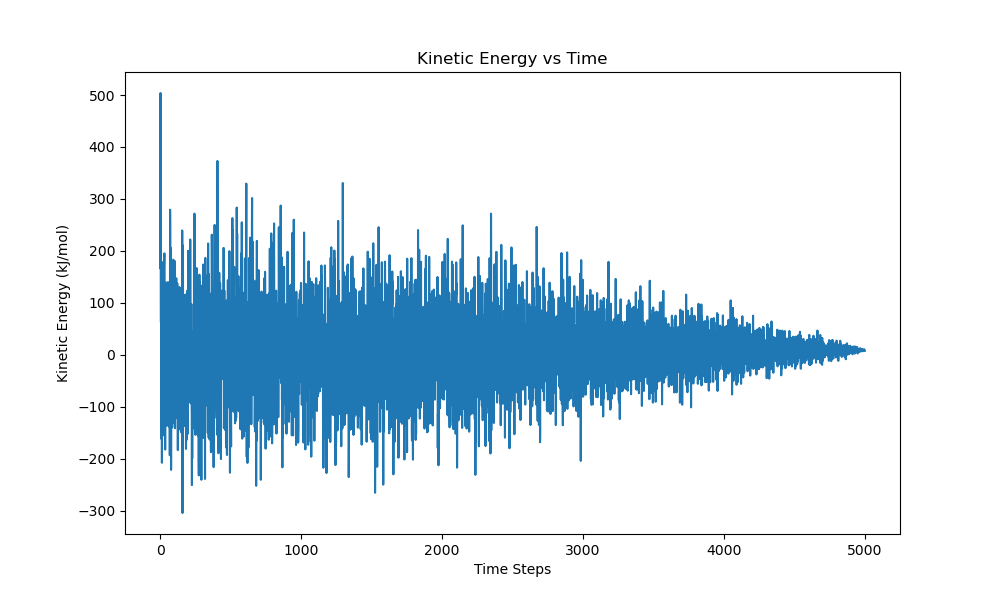
\includegraphics[scale=0.3]{kinetic_energy_plot.png}
      \caption{动能}
      \label{fig:side:a}
    \end{minipage}%
    \begin{minipage}[t]{0.5\linewidth}
      \centering
      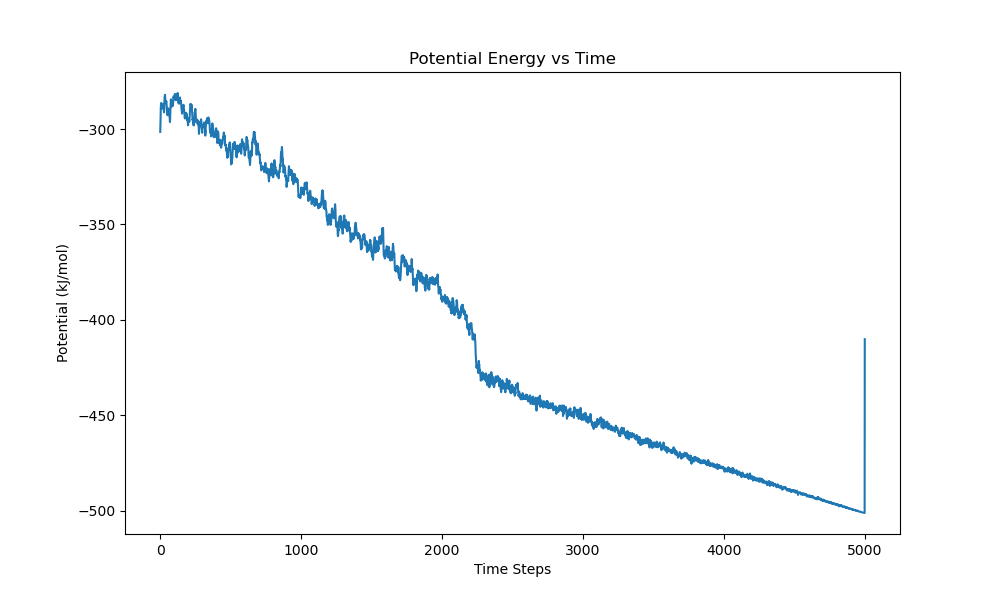
\includegraphics[scale=0.3]{potential_energy_plot.png}
      \caption{势能}
      \label{fig:side:b}
    \end{minipage}
    \begin{minipage}[t]{0.5\linewidth}
      \centering
      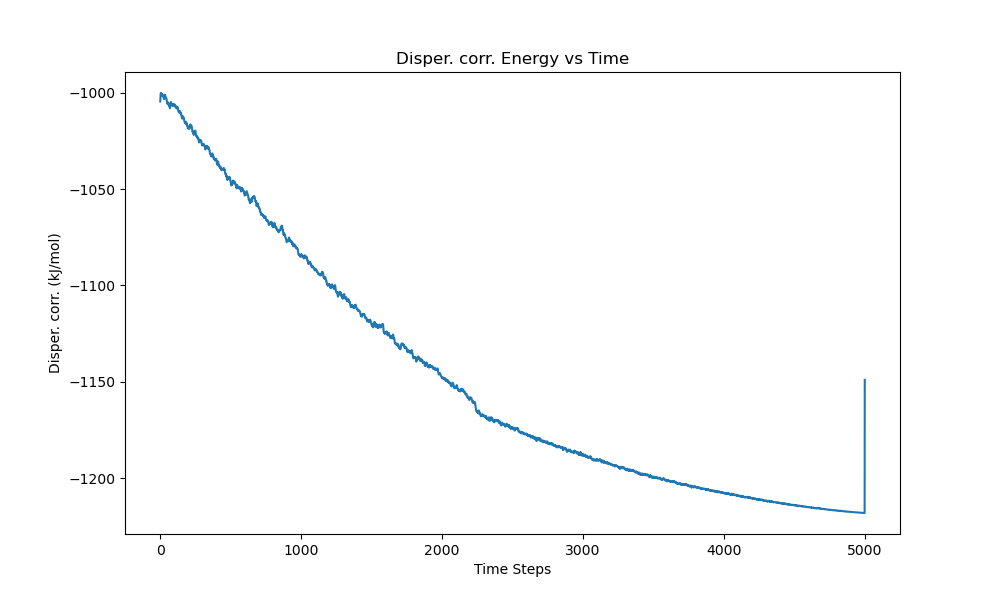
\includegraphics[scale=0.3]{disper_corr_energy_plot.png}
      \caption{分散校正能量}
      \label{fig:side:a}
    \end{minipage}%
    \begin{minipage}[t]{0.5\linewidth}
      \centering
      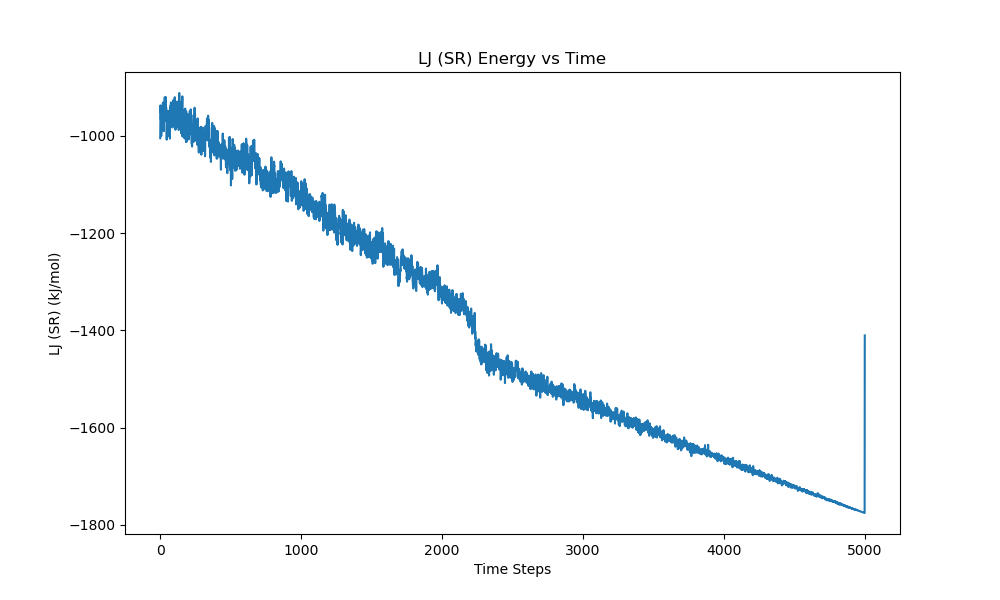
\includegraphics[scale=0.3]{lj_sr_energy_plot.png}
      \caption{Lennard-Jones相互作用能}
      \label{fig:side:b}
    \end{minipage}
    \begin{minipage}[t]{0.5\linewidth}
      \centering
      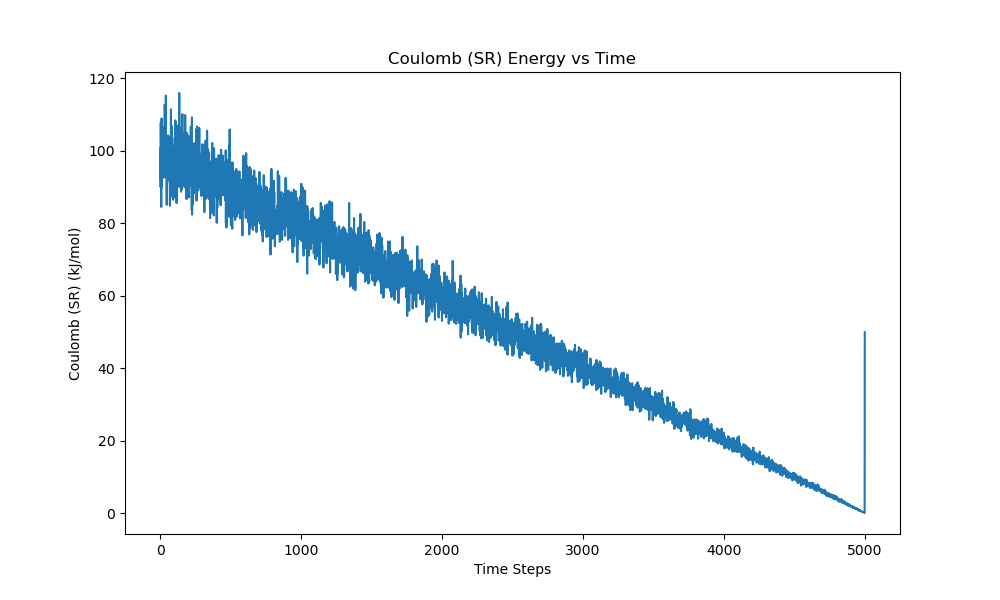
\includegraphics[scale=0.3]{coulomb_sr_energy_plot.png}
      \caption{Coulomb}
      \label{fig:side:b}
    \end{minipage}
    \begin{minipage}[t]{0.5\linewidth}
      \centering
      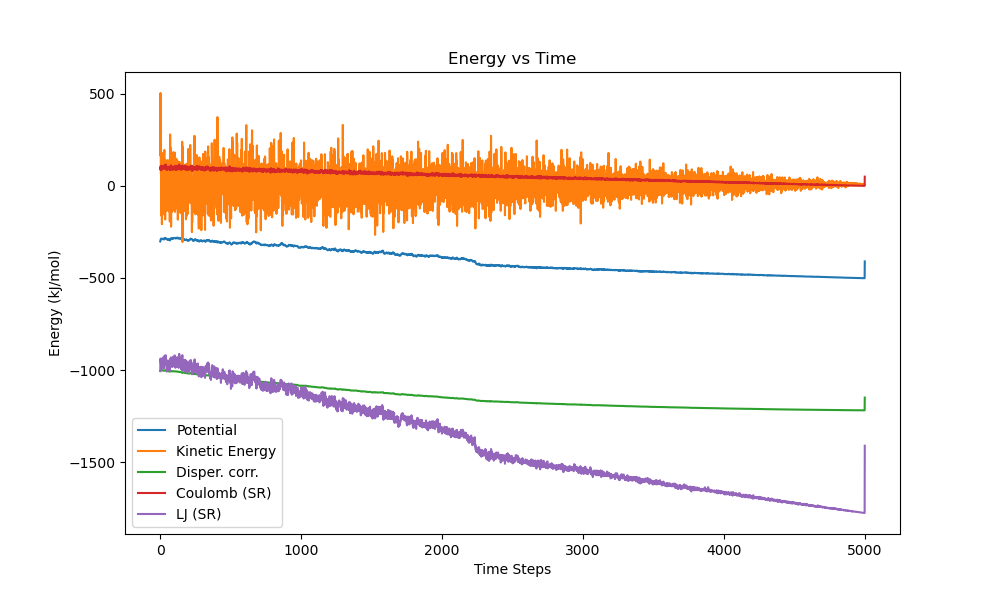
\includegraphics[scale=0.3]{analyticalfigure.png}
      \caption{总图}
      \label{fig:side:b}
    \end{minipage}
\end{figure}
根据图形观察每一项的值随着时间逐渐减小,可以得出以下可能的解释:
\\
势能逐渐减小:势能的减小可能表示系统在模拟过程中逐渐接近更稳定的能量状态。因为系统在模拟过程中发生了一系列的能量转移(温度降低),使系统朝着更低能量的状态演化。
\\
动能标准差减小:动能标准差的减小可能表示分子之间的动能差异逐渐减小,即分子的动能分布趋于均匀。这可能是由于温度随着时间的降低,使系统中的分子逐渐趋于热平衡状态。
\\
Disper的平均值减小:Disper的平均值减小可能表示系统中分子间的范德华相互作用逐渐减弱。系统在模拟过程中,分子的相对位置和取向发生了变化,导致范德华相互作用减弱。
\\
Coulomb的平均值减小:Coulomb的平均值减小可能表示系统中静电相互作用逐渐减弱。
\end{spacing}{}
\bibliographystyle{IEEEtran}
\bibliography{6thre}

\end{document}